\section{Relative Error and Graphic Analysis}
\label{error}

\subsection{Frequency Response Analysis}
\label{subsec:freqresp}

\paragraph{}
A frequency response analysis was performed using both NGSpice for simulation interpretation and GNU Octave for theorethical analysis. The graphics ploted by each one of the tools are not as similar as they would be without the several approximations made during our analysis. The causes for the absence of values for a range of frequencies in the GNU Octave graphic are already explained in the respective section. Therefore, it is important to note that the values for the maximum output gain voltage levels are really similar between the theorethical and simulation analysis. Besides that, also the lower cut-off frequencies are really close between the two analysis, making both graphics close to each other when looking to the right side of the x-axis, verifying to a good approximation to high frequency values. 

\begin{figure}[H]
\begin{subfigure}{0.5\textwidth}
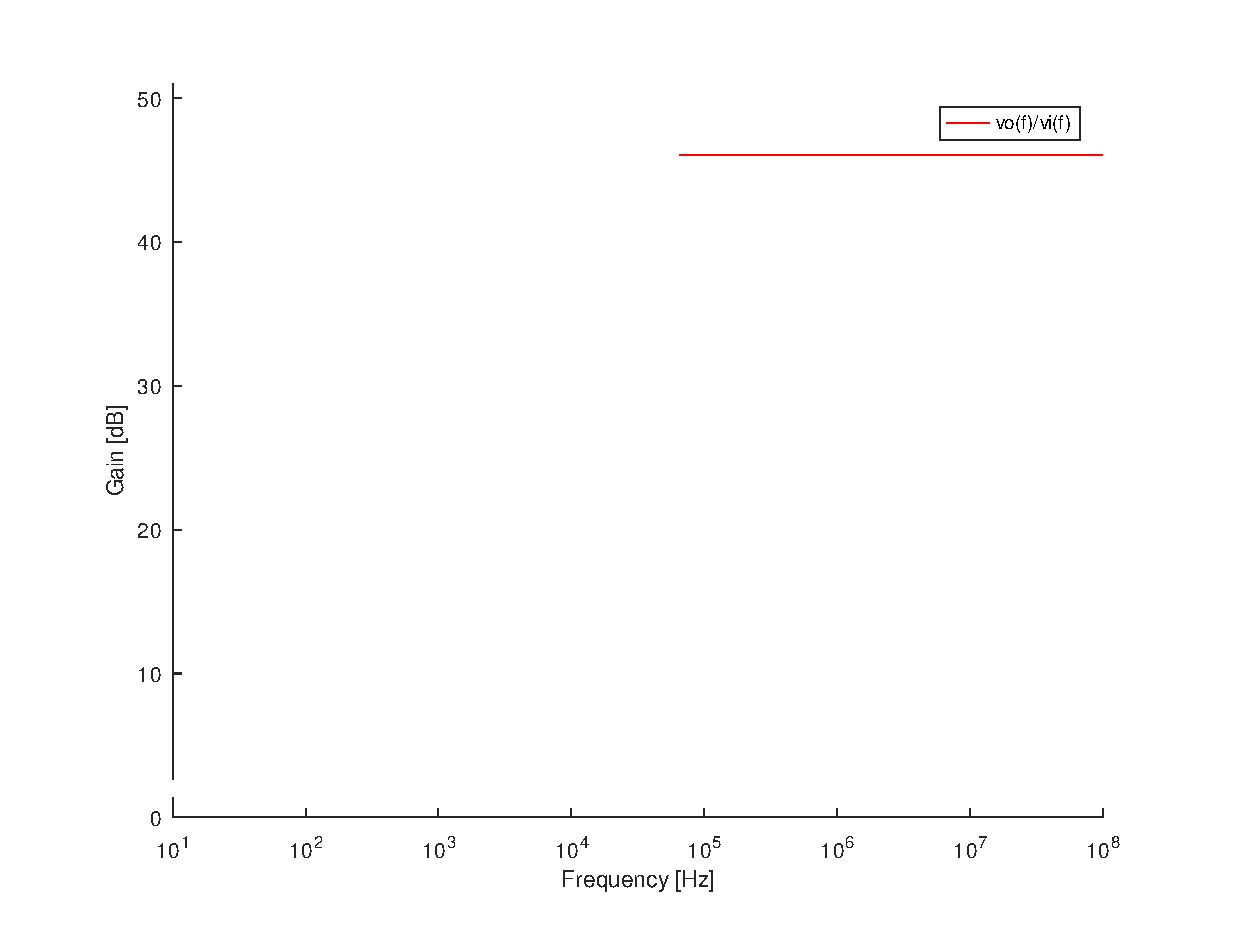
\includegraphics[width=0.9\linewidth, height=8cm]{gain.eps} 
\caption{The Output Voltage of the Output Stage of a Common Collector Amplifier, obtained using GNU Octave.}
\label{fig:theo_third}
\end{subfigure}
\begin{subfigure}{0.5\textwidth}
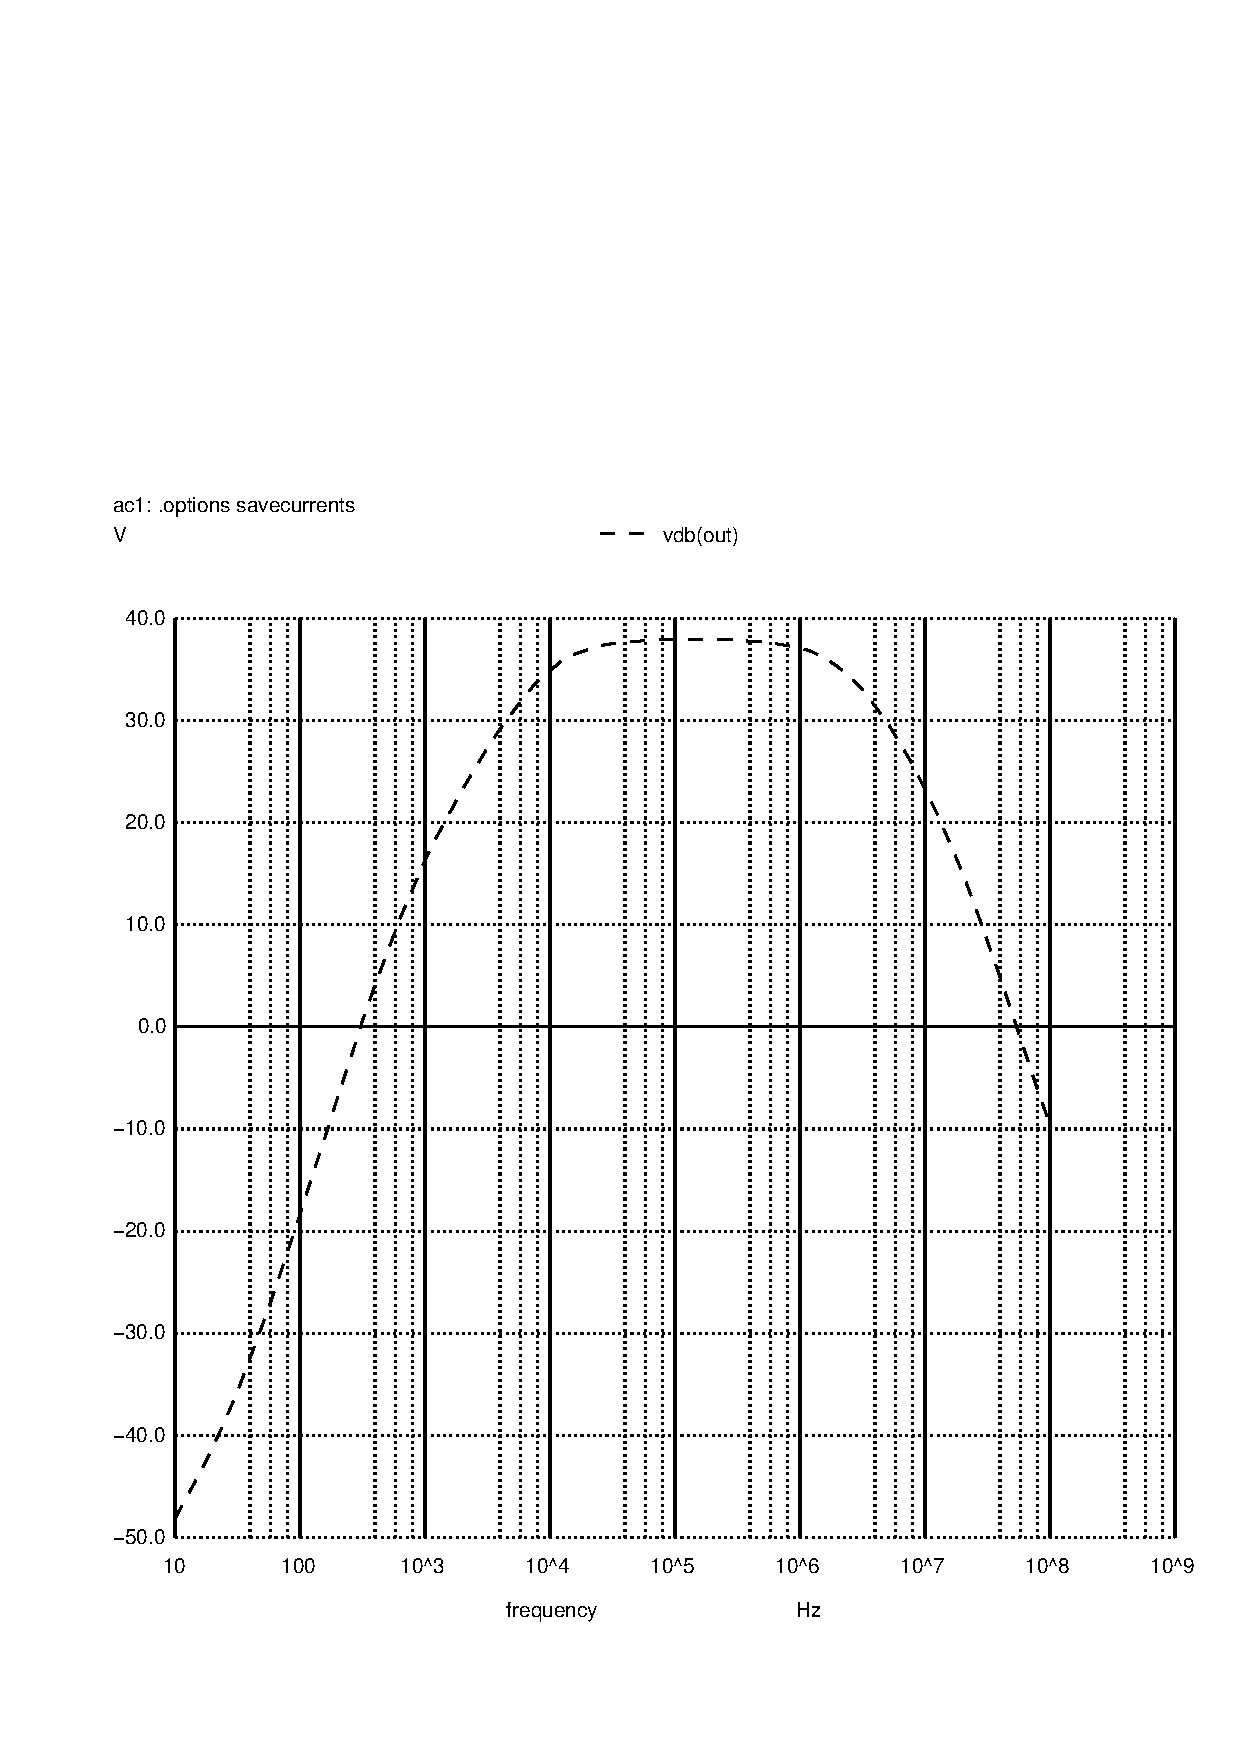
\includegraphics[width=0.8\linewidth, height=8cm]{vo2f.pdf}
\caption{The Output Voltage of the Output Stage of a Common Collector Amplifier, obtained using Ngspice.}
\label{fig:total}
\end{subfigure}
\end{figure}


\subsection{Input and Output Impedances Analysis}
\label{subsec:freqresp}

\begin{center}
   \begin{table}[H]
\resizebox{\textwidth}{!}{%
\begin{tabular}{c|c|c|c|c|c|}
\cline{3-6}
\multicolumn{2}{c}{} & \textbf{NGSpice Value} & \textbf{Octave Value} & \textbf{Relative Error} & \textbf{Percentual Error {[}\%{]}} \\ \hline
\multicolumn{1}{|c|}{\multirow{2}{*}{Gain Stage}} & Input Impedance & 574.5327 & 523.575168 & 0.08869387591 & 8.869387591 \\ \cline{2-6} 
\multicolumn{1}{|c|}{} & Output Impedance & 799.9195 & 730.963158 & 0.08620410179 & 8.620410179 \\ \hline
\multicolumn{1}{|c|}{\multirow{2}{*}{Output Stage}} & Input Impedance & 65771.74 & 78634.69849 & 0.1955696852 & 19.55696852 \\ \cline{2-6} 
\multicolumn{1}{|c|}{} & Output Impedance & 3.17595 & 3.171596 & 0.001370928384 & 0.1370928384 \\ \hline
\multicolumn{1}{c|}{} & Voltage Gain & 37.93 & 46.02225 & 0.2133469549 & 21.33469549 \\ \cline{2-6} 
\end{tabular}%
}
\end{table}
\end{center}

\paragraph{}
In the table above, we have the comparison between Octave and NGSpice values for the of the Output Voltage Gain and all the input and output impedances of the two stages of the common collector amplifier. Both the relative error and percentual error are included to make the interpretation easier. 

\paragraph{}
As we can see, some of the percentual errors are very high and thus cannot be ignored. In fact, some of the parameters defined for NGSpice circuit's components can influence in some way the impedances results being measured by those circuits. Besides that, all the formulas involved in the input and output impedances calculation process were really complex and could have minor approximations that have a final result of major differnece between the theorethical values and the simulation measured ones. A possible general explanation for these discrepancies is also that NGSpice uses a very complex transistor model, similarly to what happened in the previous laboratory assignment with the diode model, which does not have fixed parameters, and so it becames very hard for Octave to match the results. 

\subsection{Figure of Merit}
\label{subsec:Figure_of_Merit}


\paragraph{}
To end our report, we present the figure of merit. It is important to remind that this figure is obtained upon the devices and values used in Ngspice. During our work, we have performed several incremental modifications to improve the merit figure. It was really important for us to understand the influence of the coupling capacitors on the bandwidth, the purpose of the bypass capacitor in relation with the voltage gain and the effect of resistors and capacitors. 

\paragraph{}
The variation of these parameters allowed us to achieve an improved figure of merit, while trying to maximize the voltage gain and the bandwith and to minimize the cost of the circuit' components and to achieve the lowest lower cut-off frequency as posible. The values applied both in NGSpice and Octave proved to be our best options to make the figure of merit as high as possible.
